\documentclass[12pt, letterpaper, center, noupper]{uconnthesis}

\ThesisLineSpacing{2}
\usepackage[square,sort,comma,numbers]{natbib}
\renewcommand{\bibsection}{} %removes double header for bibliography section
\usepackage[varg]{txfonts}
\usepackage{wasysym}
\usepackage{graphicx}
\usepackage[colorlinks=false]{hyperref}
\graphicspath{{Figs/}}


\begin{document}

\abstract{
Insert abstract here.
}

\title{Title}
\author{Author}
\submityear{20xx}
\authorspreviousdegreelong{
B.S., Undergraduate University, 20yy\\  
M.S., University of Connecticut, 20zz
}
\authorspreviousdegreeshort{M.S.}

\MajorAdvisor{Major Advisor}
\AssociateAdvisorA{Secondary Advisor 1}
\AssociateAdvisorB{Secondary Advisor 2}

\dedication{
Dedication goes here.
}

\acknowledgements{
Insert acknowledgements here.
}

\maketitle
\frontmatter

\tableofcontents
\listoffigures
\listoftables

\mainmatter

% Chapters of the thesis

\chapter{Introduction}

Lorem ipsum dolor sit amet, consectetur adipiscing elit. Nulla at ex eget est dictum posuere a id augue. Donec vulputate ultrices tellus ultricies pellentesque. Sed sodales mi sed euismod ornare. Sed in rhoncus lectus. Integer fringilla, nunc vitae tempus suscipit, urna libero imperdiet est, ac molestie neque lacus ac nibh. Mauris erat mauris, auctor et blandit sed, fermentum eget metus. Nam fringilla ante ac viverra porttitor. Nullam sodales metus in nunc finibus pretium. Vivamus aliquet nisi ac urna consequat varius. Proin mattis leo et dui mollis porta. Phasellus molestie ex vel fermentum consequat. Maecenas et sodales mauris.

In non ex commodo, pulvinar ex ac, interdum ex. Maecenas dignissim ac neque non accumsan. Phasellus sed diam quis mauris rutrum pulvinar eu at justo. Duis dictum mattis laoreet. Quisque faucibus erat ac est fermentum pulvinar. Sed semper pulvinar metus, at convallis enim vulputate a. In hac habitasse platea dictumst. Ut sit amet viverra magna, in pretium ante. Suspendisse sit amet quam vestibulum, tincidunt purus id, sagittis risus. Aliquam id orci id sapien volutpat aliquam. Etiam congue ligula ut dui rutrum scelerisque. Suspendisse sed lacus efficitur, pulvinar urna et, eleifend nibh. Suspendisse est mi, pharetra eu nisi id, lacinia varius eros. Donec lacinia sapien imperdiet nisi malesuada, a congue velit rhoncus.

Proin pellentesque velit et mollis eleifend. Integer vel finibus purus. Ut volutpat justo ut sapien tempor finibus. Etiam maximus, turpis vitae egestas condimentum, metus purus mollis nunc, quis posuere leo arcu eu velit. Aliquam erat volutpat. Aenean vel consequat quam. Mauris viverra purus ut varius ornare. Proin dictum rhoncus ante, nec vulputate erat faucibus ut. Vestibulum blandit ultricies nulla, sit amet tempor tortor. Maecenas magna tellus, ultrices eget efficitur id, blandit eu nisi. Maecenas turpis nunc, tristique id augue vitae, dignissim pharetra nisl. Nullam vitae hendrerit orci, eu blandit turpis. Quisque diam turpis, suscipit quis ipsum id, maximus hendrerit nibh. Duis id ultrices leo.

Integer tempus dignissim feugiat. Ut ac ligula id orci aliquam fermentum et sit amet nibh. Nulla facilisi. Nam feugiat aliquet augue, dictum fermentum leo. Pellentesque habitant morbi tristique senectus et netus et malesuada fames ac turpis egestas. Proin facilisis pulvinar justo, non ultrices enim aliquam nec. Aenean felis ex, aliquet ac bibendum in, scelerisque sit amet nunc. Praesent eget leo augue. Sed sollicitudin rhoncus magna, a eleifend turpis aliquet quis. Sed vel turpis tempor, vulputate quam quis, laoreet augue. Vivamus interdum vitae felis ac varius. Maecenas ullamcorper scelerisque ligula, sed auctor lacus aliquam eu. Fusce dictum cursus diam vitae fermentum. Class aptent taciti sociosqu ad litora torquent per conubia nostra, per inceptos himenaeos.

Phasellus id mauris eu diam convallis tristique in vitae massa. Cras vitae nisi elementum, luctus magna in, sagittis nisi. Pellentesque habitant morbi tristique senectus et netus et malesuada fames ac turpis egestas. Ut metus ligula, ullamcorper sit amet lacinia vitae, dapibus in tortor. Cras condimentum, massa ut luctus scelerisque, sapien ante euismod nisl, sed malesuada quam ante luctus magna. Nulla lobortis lectus non magna suscipit, ac venenatis urna luctus. Fusce sollicitudin varius aliquet. Morbi magna elit, volutpat a lobortis ac, sollicitudin in tortor. Maecenas rhoncus, neque a blandit iaculis, augue mi iaculis lacus, ut sagittis dolor dolor vel purus.


\chapter{Analysis}

Lorem ipsum dolor sit amet, consectetur adipiscing elit. Nulla at ex eget est dictum posuere a id augue. Donec vulputate ultrices tellus ultricies pellentesque. Sed sodales mi sed euismod ornare. Sed in rhoncus lectus. Integer fringilla, nunc vitae tempus suscipit, urna libero imperdiet est, ac molestie neque lacus ac nibh. Mauris erat mauris, auctor et blandit sed, fermentum eget metus. Nam fringilla ante ac viverra porttitor. Nullam sodales metus in nunc finibus pretium. Vivamus aliquet nisi ac urna consequat varius. Proin mattis leo et dui mollis porta. Phasellus molestie ex vel fermentum consequat. Maecenas et sodales mauris.

In non ex commodo, pulvinar ex ac, interdum ex. Maecenas dignissim ac neque non accumsan. Phasellus sed diam quis mauris rutrum pulvinar eu at justo. Duis dictum mattis laoreet. Quisque faucibus erat ac est fermentum pulvinar. Sed semper pulvinar metus, at convallis enim vulputate a. In hac habitasse platea dictumst. Ut sit amet viverra magna, in pretium ante. Suspendisse sit amet quam vestibulum, tincidunt purus id, sagittis risus. Aliquam id orci id sapien volutpat aliquam. Etiam congue ligula ut dui rutrum scelerisque. Suspendisse sed lacus efficitur, pulvinar urna et, eleifend nibh. Suspendisse est mi, pharetra eu nisi id, lacinia varius eros. Donec lacinia sapien imperdiet nisi malesuada, a congue velit rhoncus.


\begin{table}[t]
\begin{center}
\begin{tabular}{ |c|c|c| } 
 \hline
 cell1 & cell2 & cell3 \\ 
 cell4 & cell5 & cell6 \\ 
 cell7 & cell8 & cell9 \\ 
 \hline
\end{tabular}
\caption[Example Table]{An example of a table}
	\label{example_table} 
\end{center}
\end{table}

Proin pellentesque velit et mollis eleifend. Integer vel finibus purus. Ut volutpat justo ut sapien tempor finibus. Etiam maximus, turpis vitae egestas condimentum, metus purus mollis nunc, quis posuere leo arcu eu velit. Aliquam erat volutpat. Aenean vel consequat quam. Mauris viverra purus ut varius ornare. Proin dictum rhoncus ante, nec vulputate erat faucibus ut. Vestibulum blandit ultricies nulla, sit amet tempor tortor. Maecenas magna tellus, ultrices eget efficitur id, blandit eu nisi. Maecenas turpis nunc, tristique id augue vitae, dignissim pharetra nisl. Nullam vitae hendrerit orci, eu blandit turpis. Quisque diam turpis, suscipit quis ipsum id, maximus hendrerit nibh. Duis id ultrices leo.

Integer tempus dignissim feugiat. Ut ac ligula id orci aliquam fermentum et sit amet nibh. Nulla facilisi. Nam feugiat aliquet augue, dictum fermentum leo. Pellentesque habitant morbi tristique senectus et netus et malesuada fames ac turpis egestas. Proin facilisis pulvinar justo, non ultrices enim aliquam nec. Aenean felis ex, aliquet ac bibendum in, scelerisque sit amet nunc. Praesent eget leo augue. Sed sollicitudin rhoncus magna, a eleifend turpis aliquet quis. Sed vel turpis tempor, vulputate quam quis, laoreet augue. Vivamus interdum vitae felis ac varius. Maecenas ullamcorper scelerisque ligula, sed auctor lacus aliquam eu. Fusce dictum cursus diam vitae fermentum. Class aptent taciti sociosqu ad litora torquent per conubia nostra, per inceptos himenaeos.

Phasellus id mauris eu diam convallis tristique in vitae massa. Cras vitae nisi elementum, luctus magna in, sagittis nisi. Pellentesque habitant morbi tristique senectus et netus et malesuada fames ac turpis egestas. Ut metus ligula, ullamcorper sit amet lacinia vitae, dapibus in tortor. Cras condimentum, massa ut luctus scelerisque, sapien ante euismod nisl, sed malesuada quam ante luctus magna. Nulla lobortis lectus non magna suscipit, ac venenatis urna luctus. Fusce sollicitudin varius aliquet. Morbi magna elit, volutpat a lobortis ac, sollicitudin in tortor. Maecenas rhoncus, neque a blandit iaculis, augue mi iaculis lacus, ut sagittis dolor dolor vel purus.



\chapter{Results}

Lorem ipsum dolor sit amet, consectetur adipiscing elit. Nulla at ex eget est dictum posuere a id augue. Donec vulputate ultrices tellus ultricies pellentesque. Sed sodales mi sed euismod ornare. Sed in rhoncus lectus. Integer fringilla, nunc vitae tempus suscipit, urna libero imperdiet est, ac molestie neque lacus ac nibh. Mauris erat mauris, auctor et blandit sed, fermentum eget metus. Nam fringilla ante ac viverra porttitor. Nullam sodales metus in nunc finibus pretium. Vivamus aliquet nisi ac urna consequat varius. Proin mattis leo et dui mollis porta. Phasellus molestie ex vel fermentum consequat. Maecenas et sodales mauris.

In non ex commodo, pulvinar ex ac, interdum ex. Maecenas dignissim ac neque non accumsan. Phasellus sed diam quis mauris rutrum pulvinar eu at justo. Duis dictum mattis laoreet. Quisque faucibus erat ac est fermentum pulvinar. Sed semper pulvinar metus, at convallis enim vulputate a. In hac habitasse platea dictumst. Ut sit amet viverra magna, in pretium ante. Suspendisse sit amet quam vestibulum, tincidunt purus id, sagittis risus. Aliquam id orci id sapien volutpat aliquam. Etiam congue ligula ut dui rutrum scelerisque. Suspendisse sed lacus efficitur, pulvinar urna et, eleifend nibh. Suspendisse est mi, pharetra eu nisi id, lacinia varius eros. Donec lacinia sapien imperdiet nisi malesuada, a congue velit rhoncus.


\begin{figure}
	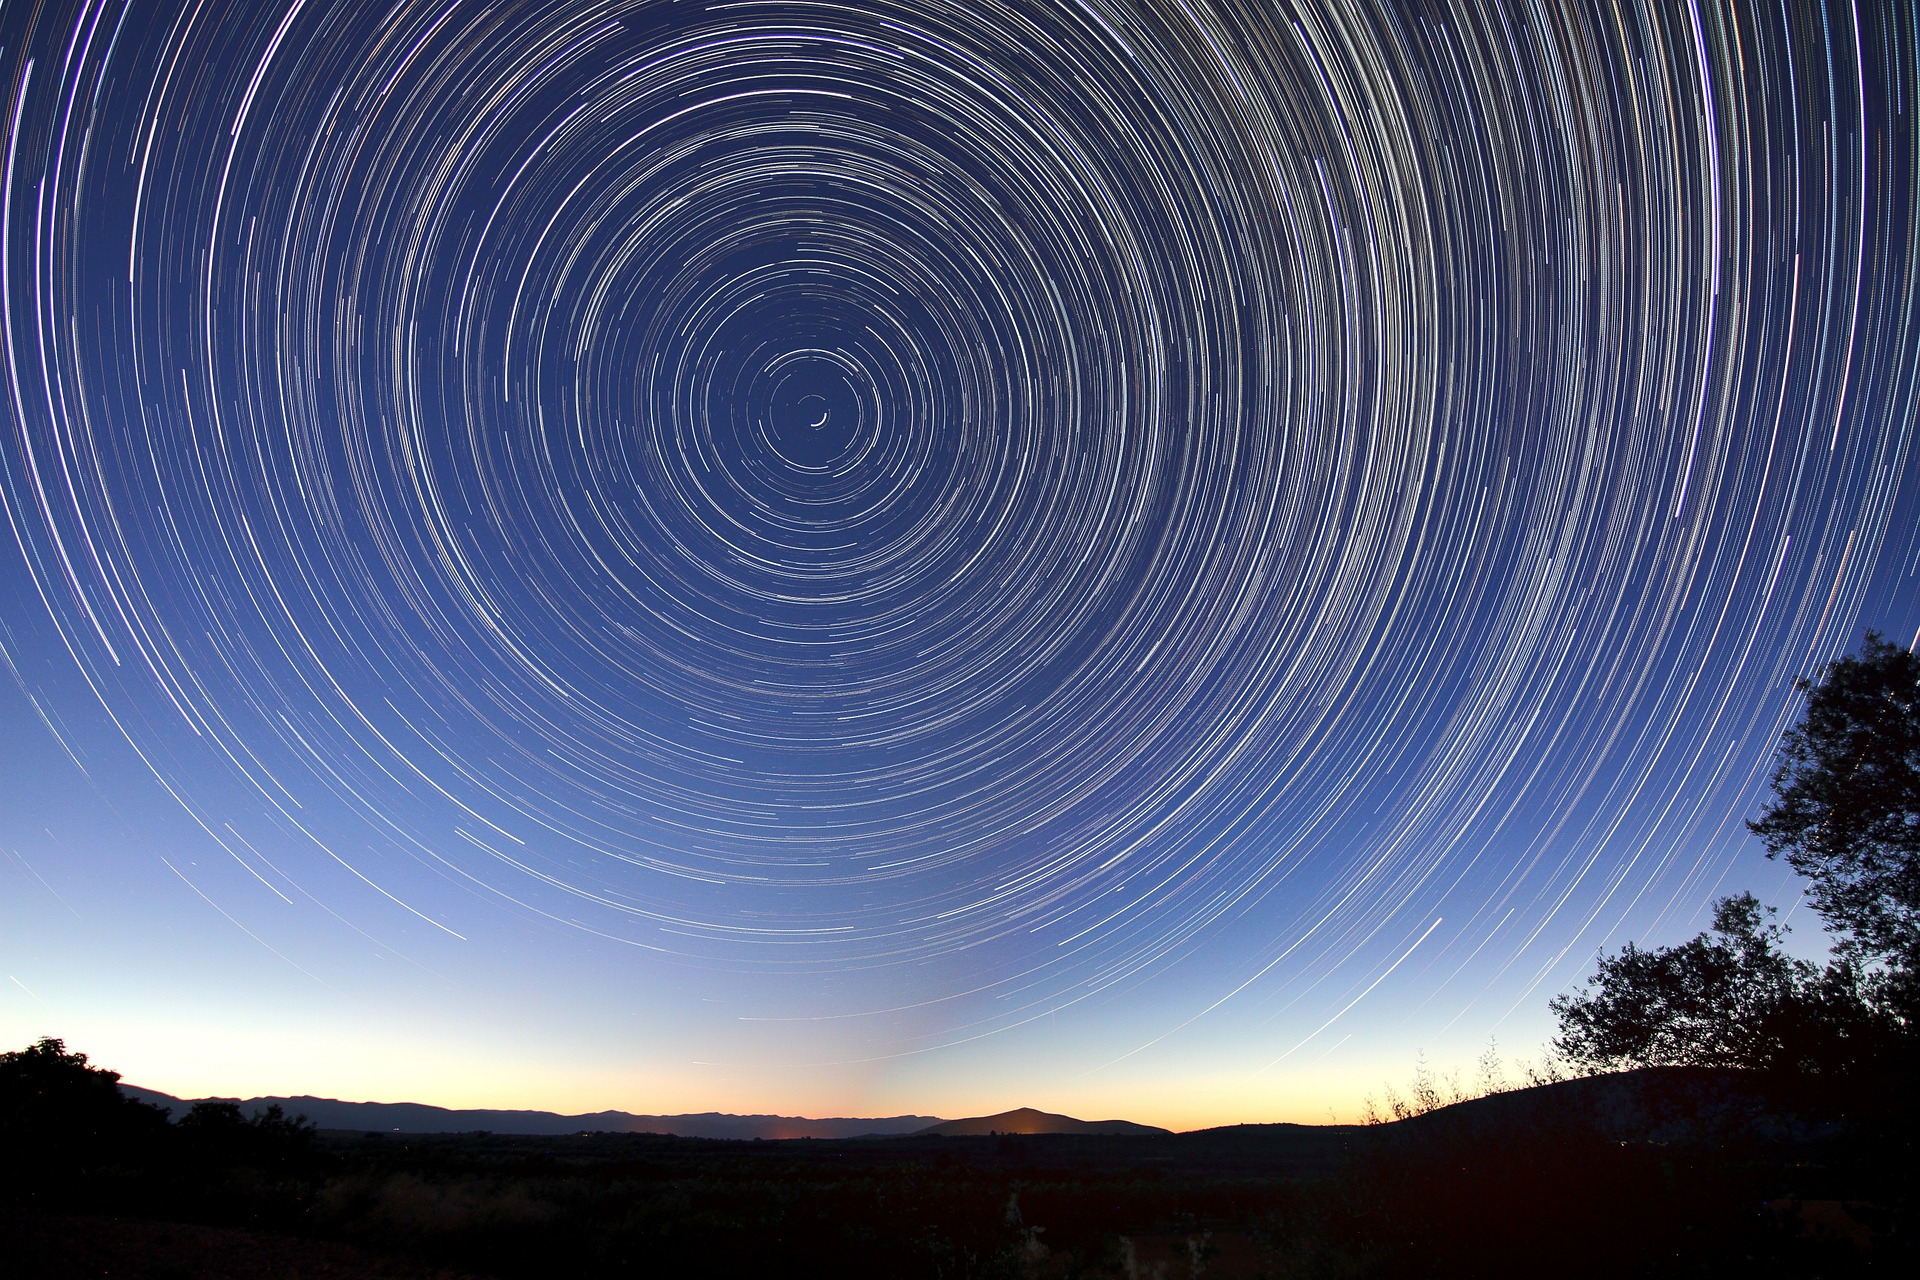
\includegraphics[width=1.0\textwidth]{star_trails.jpg} 
	\caption[Example Figure]{An example of figure.}
\label{example_figure}
\end{figure}

Proin pellentesque velit et mollis eleifend. Integer vel finibus purus. Ut volutpat justo ut sapien tempor finibus. Etiam maximus, turpis vitae egestas condimentum, metus purus mollis nunc, quis posuere leo arcu eu velit. Aliquam erat volutpat. Aenean vel consequat quam. Mauris viverra purus ut varius ornare. Proin dictum rhoncus ante, nec vulputate erat faucibus ut. Vestibulum blandit ultricies nulla, sit amet tempor tortor. Maecenas magna tellus, ultrices eget efficitur id, blandit eu nisi. Maecenas turpis nunc, tristique id augue vitae, dignissim pharetra nisl. Nullam vitae hendrerit orci, eu blandit turpis. Quisque diam turpis, suscipit quis ipsum id, maximus hendrerit nibh. Duis id ultrices leo.

Integer tempus dignissim feugiat. Ut ac ligula id orci aliquam fermentum et sit amet nibh. Nulla facilisi. Nam feugiat aliquet augue, dictum fermentum leo. Pellentesque habitant morbi tristique senectus et netus et malesuada fames ac turpis egestas. Proin facilisis pulvinar justo, non ultrices enim aliquam nec. Aenean felis ex, aliquet ac bibendum in, scelerisque sit amet nunc. Praesent eget leo augue. Sed sollicitudin rhoncus magna, a eleifend turpis aliquet quis. Sed vel turpis tempor, vulputate quam quis, laoreet augue. Vivamus interdum vitae felis ac varius. Maecenas ullamcorper scelerisque ligula, sed auctor lacus aliquam eu. Fusce dictum cursus diam vitae fermentum. Class aptent taciti sociosqu ad litora torquent per conubia nostra, per inceptos himenaeos.

Phasellus id mauris eu diam convallis tristique in vitae massa. Cras vitae nisi elementum, luctus magna in, sagittis nisi. Pellentesque habitant morbi tristique senectus et netus et malesuada fames ac turpis egestas. Ut metus ligula, ullamcorper sit amet lacinia vitae, dapibus in tortor. Cras condimentum, massa ut luctus scelerisque, sapien ante euismod nisl, sed malesuada quam ante luctus magna. Nulla lobortis lectus non magna suscipit, ac venenatis urna luctus. Fusce sollicitudin varius aliquet. Morbi magna elit, volutpat a lobortis ac, sollicitudin in tortor. Maecenas rhoncus, neque a blandit iaculis, augue mi iaculis lacus, ut sagittis dolor dolor vel purus.


\chapter{Discussion}

Lorem ipsum dolor sit amet, consectetur adipiscing elit. Nulla at ex eget est dictum posuere a id augue. Donec vulputate ultrices tellus ultricies pellentesque. Sed sodales mi sed euismod ornare. Sed in rhoncus lectus. Integer fringilla, nunc vitae tempus suscipit, urna libero imperdiet est, ac molestie neque lacus ac nibh. Mauris erat mauris, auctor et blandit sed, fermentum eget metus. Nam fringilla ante ac viverra porttitor. Nullam sodales metus in nunc finibus pretium. Vivamus aliquet nisi ac urna consequat varius. Proin mattis leo et dui mollis porta. Phasellus molestie ex vel fermentum consequat. Maecenas et sodales mauris.

In non ex commodo, pulvinar ex ac, interdum ex. Maecenas dignissim ac neque non accumsan. Phasellus sed diam quis mauris rutrum pulvinar eu at justo. Duis dictum mattis laoreet. Quisque faucibus erat ac est fermentum pulvinar. Sed semper pulvinar metus, at convallis enim vulputate a. In hac habitasse platea dictumst. Ut sit amet viverra magna, in pretium ante. Suspendisse sit amet quam vestibulum, tincidunt purus id, sagittis risus. Aliquam id orci id sapien volutpat aliquam. Etiam congue ligula ut dui rutrum scelerisque. Suspendisse sed lacus efficitur, pulvinar urna et, eleifend nibh \citep{example_ref1}. Suspendisse est mi, pharetra eu nisi id, lacinia varius eros. Donec lacinia sapien imperdiet nisi malesuada, a congue velit rhoncus.

Proin pellentesque velit et mollis eleifend. Integer vel finibus purus. Ut volutpat justo ut sapien tempor finibus. Etiam maximus, turpis vitae egestas condimentum, metus purus mollis nunc, quis posuere leo arcu eu velit. Aliquam erat volutpat. Aenean vel consequat quam. Mauris viverra purus ut varius ornare. Proin dictum rhoncus ante, nec vulputate erat faucibus ut. Vestibulum blandit ultricies nulla, sit amet tempor tortor. Maecenas magna tellus, ultrices eget efficitur id, blandit eu nisi. Maecenas turpis nunc, tristique id augue vitae, dignissim pharetra nisl. Nullam vitae hendrerit orci, eu blandit turpis. Quisque diam turpis, suscipit quis ipsum id, maximus hendrerit nibh. Duis id ultrices leo.

Integer tempus dignissim feugiat. Ut ac ligula id orci aliquam fermentum et sit amet nibh. Nulla facilisi. Nam feugiat aliquet augue, dictum fermentum leo. Pellentesque habitant morbi tristique senectus et netus et malesuada fames ac turpis egestas. Proin facilisis pulvinar justo, non ultrices enim aliquam nec. Aenean felis ex, aliquet ac bibendum in, scelerisque sit amet nunc. Praesent eget leo augue. Sed sollicitudin rhoncus magna, a eleifend turpis aliquet quis. Sed vel turpis tempor, vulputate quam quis, laoreet augue \citep{example_ref2}. Vivamus interdum vitae felis ac varius. Maecenas ullamcorper scelerisque ligula, sed auctor lacus aliquam eu. Fusce dictum cursus diam vitae fermentum. Class aptent taciti sociosqu ad litora torquent per conubia nostra, per inceptos himenaeos.

Phasellus id mauris eu diam convallis tristique in vitae massa. Cras vitae nisi elementum, luctus magna in, sagittis nisi. Pellentesque habitant morbi tristique senectus et netus et malesuada fames ac turpis egestas. Ut metus ligula, ullamcorper sit amet lacinia vitae, dapibus in tortor. Cras condimentum, massa ut luctus scelerisque, sapien ante euismod nisl, sed malesuada quam ante luctus magna. Nulla lobortis lectus non magna suscipit, ac venenatis urna luctus. Fusce sollicitudin varius aliquet. Morbi magna elit, volutpat a lobortis ac, sollicitudin in tortor. Maecenas rhoncus, neque a blandit iaculis, augue mi iaculis lacus, ut sagittis dolor dolor vel purus.



\chapter{Conclusions}

Lorem ipsum dolor sit amet, consectetur adipiscing elit. Nulla at ex eget est dictum posuere a id augue. Donec vulputate ultrices tellus ultricies pellentesque. Sed sodales mi sed euismod ornare. Sed in rhoncus lectus. Integer fringilla, nunc vitae tempus suscipit, urna libero imperdiet est, ac molestie neque lacus ac nibh. Mauris erat mauris, auctor et blandit sed, fermentum eget metus. Nam fringilla ante ac viverra porttitor. Nullam sodales metus in nunc finibus pretium. Vivamus aliquet nisi ac urna consequat varius. Proin mattis leo et dui mollis porta. Phasellus molestie ex vel fermentum consequat. Maecenas et sodales mauris.

In non ex commodo, pulvinar ex ac, interdum ex. Maecenas dignissim ac neque non accumsan. Phasellus sed diam quis mauris rutrum pulvinar eu at justo. Duis dictum mattis laoreet. Quisque faucibus erat ac est fermentum pulvinar. Sed semper pulvinar metus, at convallis enim vulputate a. In hac habitasse platea dictumst. Ut sit amet viverra magna, in pretium ante. Suspendisse sit amet quam vestibulum, tincidunt purus id, sagittis risus. Aliquam id orci id sapien volutpat aliquam. Etiam congue ligula ut dui rutrum scelerisque. Suspendisse sed lacus efficitur, pulvinar urna et, eleifend nibh. Suspendisse est mi, pharetra eu nisi id, lacinia varius eros. Donec lacinia sapien imperdiet nisi malesuada, a congue velit rhoncus.

Proin pellentesque velit et mollis eleifend. Integer vel finibus purus. Ut volutpat justo ut sapien tempor finibus. Etiam maximus, turpis vitae egestas condimentum, metus purus mollis nunc, quis posuere leo arcu eu velit. Aliquam erat volutpat. Aenean vel consequat quam. Mauris viverra purus ut varius ornare. Proin dictum rhoncus ante, nec vulputate erat faucibus ut. Vestibulum blandit ultricies nulla, sit amet tempor tortor. Maecenas magna tellus, ultrices eget efficitur id, blandit eu nisi. Maecenas turpis nunc, tristique id augue vitae, dignissim pharetra nisl. Nullam vitae hendrerit orci, eu blandit turpis. Quisque diam turpis, suscipit quis ipsum id, maximus hendrerit nibh. Duis id ultrices leo.

Integer tempus dignissim feugiat. Ut ac ligula id orci aliquam fermentum et sit amet nibh. Nulla facilisi. Nam feugiat aliquet augue, dictum fermentum leo. Pellentesque habitant morbi tristique senectus et netus et malesuada fames ac turpis egestas. Proin facilisis pulvinar justo, non ultrices enim aliquam nec. Aenean felis ex, aliquet ac bibendum in, scelerisque sit amet nunc. Praesent eget leo augue. Sed sollicitudin rhoncus magna, a eleifend turpis aliquet quis. Sed vel turpis tempor, vulputate quam quis, laoreet augue. Vivamus interdum vitae felis ac varius. Maecenas ullamcorper scelerisque ligula, sed auctor lacus aliquam eu. Fusce dictum cursus diam vitae fermentum. Class aptent taciti sociosqu ad litora torquent per conubia nostra, per inceptos himenaeos.

Phasellus id mauris eu diam convallis tristique in vitae massa. Cras vitae nisi elementum, luctus magna in, sagittis nisi. Pellentesque habitant morbi tristique senectus et netus et malesuada fames ac turpis egestas. Ut metus ligula, ullamcorper sit amet lacinia vitae, dapibus in tortor. Cras condimentum, massa ut luctus scelerisque, sapien ante euismod nisl, sed malesuada quam ante luctus magna. Nulla lobortis lectus non magna suscipit, ac venenatis urna luctus. Fusce sollicitudin varius aliquet. Morbi magna elit, volutpat a lobortis ac, sollicitudin in tortor. Maecenas rhoncus, neque a blandit iaculis, augue mi iaculis lacus, ut sagittis dolor dolor vel purus.



% All the references are located in here
\chapter*{Bibliography}
\addcontentsline{toc}{chapter}{Bibliography}

\bibliographystyle{uconn_unsrtnat}
\singlespacing\bibliography{bibliography} %link to bibtex file here


% Appendices: Place them after references
\appendix

\chapter{Additional Material}

Lorem ipsum dolor sit amet, consectetur adipiscing elit. Nulla at ex eget est dictum posuere a id augue. Donec vulputate ultrices tellus ultricies pellentesque. Sed sodales mi sed euismod ornare. Sed in rhoncus lectus. Integer fringilla, nunc vitae tempus suscipit, urna libero imperdiet est, ac molestie neque lacus ac nibh. Mauris erat mauris, auctor et blandit sed, fermentum eget metus. Nam fringilla ante ac viverra porttitor. Nullam sodales metus in nunc finibus pretium. Vivamus aliquet nisi ac urna consequat varius. Proin mattis leo et dui mollis porta. Phasellus molestie ex vel fermentum consequat. Maecenas et sodales mauris.

In non ex commodo, pulvinar ex ac, interdum ex. Maecenas dignissim ac neque non accumsan. Phasellus sed diam quis mauris rutrum pulvinar eu at justo. Duis dictum mattis laoreet. Quisque faucibus erat ac est fermentum pulvinar. Sed semper pulvinar metus, at convallis enim vulputate a. In hac habitasse platea dictumst. Ut sit amet viverra magna, in pretium ante. Suspendisse sit amet quam vestibulum, tincidunt purus id, sagittis risus. Aliquam id orci id sapien volutpat aliquam. Etiam congue ligula ut dui rutrum scelerisque. Suspendisse sed lacus efficitur, pulvinar urna et, eleifend nibh. Suspendisse est mi, pharetra eu nisi id, lacinia varius eros. Donec lacinia sapien imperdiet nisi malesuada, a congue velit rhoncus.

Proin pellentesque velit et mollis eleifend. Integer vel finibus purus. Ut volutpat justo ut sapien tempor finibus. Etiam maximus, turpis vitae egestas condimentum, metus purus mollis nunc, quis posuere leo arcu eu velit. Aliquam erat volutpat. Aenean vel consequat quam. Mauris viverra purus ut varius ornare. Proin dictum rhoncus ante, nec vulputate erat faucibus ut. Vestibulum blandit ultricies nulla, sit amet tempor tortor. Maecenas magna tellus, ultrices eget efficitur id, blandit eu nisi. Maecenas turpis nunc, tristique id augue vitae, dignissim pharetra nisl. Nullam vitae hendrerit orci, eu blandit turpis. Quisque diam turpis, suscipit quis ipsum id, maximus hendrerit nibh. Duis id ultrices leo.

Integer tempus dignissim feugiat. Ut ac ligula id orci aliquam fermentum et sit amet nibh. Nulla facilisi. Nam feugiat aliquet augue, dictum fermentum leo. Pellentesque habitant morbi tristique senectus et netus et malesuada fames ac turpis egestas. Proin facilisis pulvinar justo, non ultrices enim aliquam nec. Aenean felis ex, aliquet ac bibendum in, scelerisque sit amet nunc. Praesent eget leo augue. Sed sollicitudin rhoncus magna, a eleifend turpis aliquet quis. Sed vel turpis tempor, vulputate quam quis, laoreet augue. Vivamus interdum vitae felis ac varius. Maecenas ullamcorper scelerisque ligula, sed auctor lacus aliquam eu. Fusce dictum cursus diam vitae fermentum. Class aptent taciti sociosqu ad litora torquent per conubia nostra, per inceptos himenaeos.

Phasellus id mauris eu diam convallis tristique in vitae massa. Cras vitae nisi elementum, luctus magna in, sagittis nisi. Pellentesque habitant morbi tristique senectus et netus et malesuada fames ac turpis egestas. Ut metus ligula, ullamcorper sit amet lacinia vitae, dapibus in tortor. Cras condimentum, massa ut luctus scelerisque, sapien ante euismod nisl, sed malesuada quam ante luctus magna. Nulla lobortis lectus non magna suscipit, ac venenatis urna luctus. Fusce sollicitudin varius aliquet. Morbi magna elit, volutpat a lobortis ac, sollicitudin in tortor. Maecenas rhoncus, neque a blandit iaculis, augue mi iaculis lacus, ut sagittis dolor dolor vel purus.


%\input{Chapters/Table.tex}

\end{document}






